\documentclass[twocolumn,gsifonts,twoside]{gsipaper}
\usepackage{a4wide,gsiindex,helvet}
\usepackage[english]{babel}
\usepackage{amsmath,amsfonts,amssymb,verbatim,float}
\usepackage[]{graphicx} % Graphic files: pdf or jpg
\usepackage{booktabs}
\usepackage{subfig}

% \usepackage{natbib}
\usepackage{hyperref}

\graphicspath{{./Images/}}


% TODO spelling check

\begin{document}
\title{\textbf{Investigation of latent space structure}}

\abstract{ % TODO abstact dopo aver riletto Question
Qlo che ho fatto
Manifold hypothesis
how true is it relating
}

\shortauthor{Lancione, Jacopo}
\shorttitle{Deep Learning Final Project}

\author{Jacopo Lancione}
\address{Università di Torino, jacopo.lancione@edu.unito.it}

\maketitle

\section{Question and insights}
% TODO sii 1 filo - roboante
This work revolves around the latent representiation developed with autoencoders and how far the insight of the manifold hypothesis can be pushed with this respect. In other words, is there really a connection between the latent representation build by autoencoders and the supposed data manifold?

First, some comments on the intuition of the data manifold, because they will be the lighthouse of the following analysis. Intuition suggests that within the space of the features the actual meaningful data lies on an embedded manifold. So the data is expected to have some kind of structure. The easiest case to inspect this supposed structure is to use data that already suggests part of it and then verify if this is preserved in the representation developed by the autoencoder. For the sake of concreteness let us develop straight away the example at the basis of this work. The dataset used is MNIST, the feature space is the $28\times28$-dimensional space of all possible grey scale images. The data is hand-written digits and some structure of the data is suggested by the labels, i.e. the digits. Now the key argument: by moving on the supposed data manifold one would expect to reach all the instances of the same digit without crossing to another digit. Therefore different digits should be separated on the learned representation of such manifold, since starting from a data point labelled with digit 2 it would be awkward to be forced to go through a region of 7s to reach another instance of digit 2. This is the structure one would see preserved in a somewhat faithful representation of the data manifold.

The proposed argument infers that representations such as fig.~\ref{fig:vae} have little to do with the supposed data manifold, since in the encoding process they loose part of the structure of the data, which could result in an inefficient latent code.

\begin{figure}
  \centering
  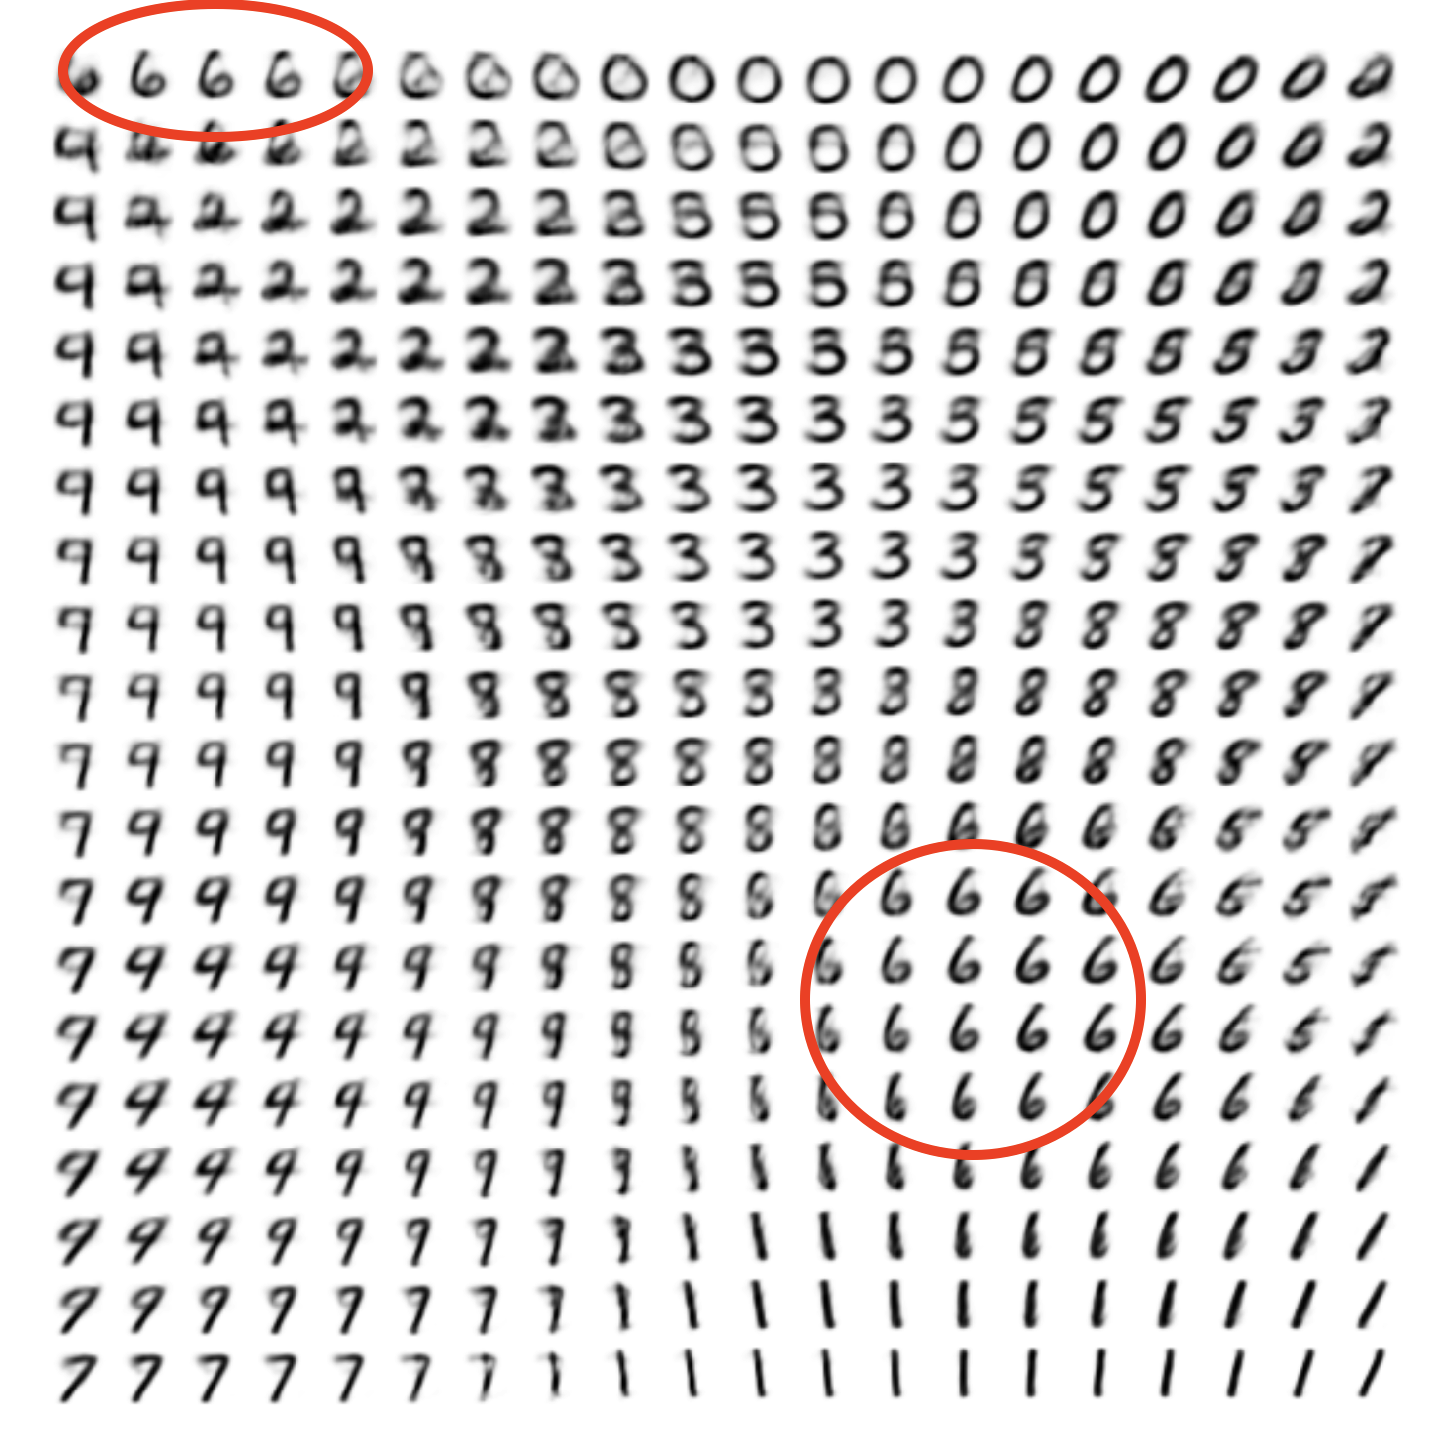
\includegraphics[width=.6\linewidth]{image_from_vae.png}
  \caption{2-dimensional latent representation build with a variational autoencoder \cite{Kingma2022}. The digit 6 appears at least in two different disconnected regions.}
  \label{fig:vae}
\end{figure}


\section{Methods}
To have a better understanding of the analysis I decided to fix the latent dimension for all the models to 2. There are two main reasons for this: first I wanted to keep a solid understanding of the latent space being able to visualize it without any sort of projection; second because the dimension of the data manifold is unknown, but it has to at least take into account for some degree of rotations and strectches of the digits' images. These are supposed to be the main transformations that map data points into data points. Thus, as a rough approximation, 2 is supposed to be a sufficient dimension to preserve at least the major structures in the data of the single digit. But, to tackle the question posed initially, at least 2 digits are needed to study how well the latent representations keeps them separated.

To sum up, I considered 2 labels at a time from dataset MNIST of hand-written digits; trained a model able to map the data to a 2 dimensional space; studied the representation. The analysis was carried on for three different models: a PCA algorithm, an autoencoder and a denoising autoencoder (fig.~\ref{fig:denoising_ae}). To compare the latent representations the metric chosen is the silhouette $s$ score \cite{Rousseeuw1987}. 
\begin{figure}
  \centering
  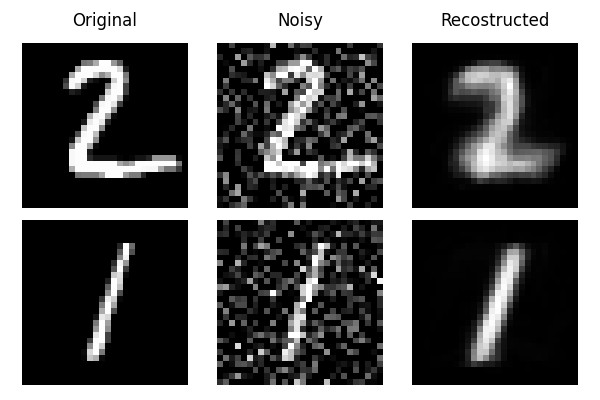
\includegraphics[width=.75\linewidth]{denoising_ae.png}
  \caption{Denoising autoencoder recostructed images}
  \label{fig:denoising_ae}
\end{figure}

\subsection{Autoencoder architecture}
The two kinds of autoencoders considered, normal and denoising share both the architecture and the training procedure\footnote{The code to reproduce all the results is hosted in the repository \url{https://github.com/jlancione/DeepLearningProject}}. The starting point is the choice to fix the latent space dimension to 2. This forces the network to compress the input to a very short code. Thus, there is no need to ask for sparsity on the latent space, since trying to impose constraints on the only two neurons would worsen the performance, pointing towards MSE as loss function. This choice to avoid regularization goes on to the encoder and decoder, summarized in table~\ref{tab:architecture}, whose weights are not tied. Again, this is because the latent space dimensionality is already a strong enough constraint imposed to the net to learn an efficient representation. Moreover, I observed that adding other hidden layers for a more gradual compression does not performs as good as the architecture proposed in table~\ref{tab:architecture}.

All this reasoning relies on the validation loss as model evaluation metric. 

\begin{table}
  \centering
  \begin{tabular}{c c}
    \toprule
    \multicolumn{2}{c}{Fully connected layers} \\ 
    \midrule
    \textbf{Encoder} & $28\times28 \mapsto 128 \mapsto 32 \mapsto 2$ \\
    \textbf{Decoder} & $2 \mapsto 32 \mapsto 128 \mapsto 28\times28$ \\
    \bottomrule
  \end{tabular}
  \caption{Autoencoder architecture summary (the denoising case uses the same one). Encoder and decoder weights are not tied. Training specifics: Adam as optimizer with learning rate $lr=10^{-2}$, weight decay $=10^{-6}$. For the denoising version the gaussian noise factor is 0.3}
  \label{tab:architecture}
\end{table}


\subsection{Activation function}
Between the fully connected layers the preferred activation function is $\tanh$. With the same architecture, it performs slightly better than ReLU, referring to the validation loss, but it is able to provide higher quality representations with a better separation of the labelled data. The reason lies in the hard cut off of the ReLU that causes most of the data to gather around the origin making the clustering harder. This proved to be especially true in the case of hard to distinguish couples of digits, for example 1 and 7, where the network with ReLU recostructs always a cloudy average digit, while the one with $\tanh$ manages not only to reconstruct them but also to cluster them.

\subsection{PCA}
The algorithm is implemented as a linear autoencoder, since it is known that PCA is the best linear autoencoder provided to impose teid weights. Therefore, the code is the same of the autoencoder implementation, removing activation functions and hidden layers keeping the 2 dimensional latent space. This leads to the same latent space representation as the classical implementation of PCA, but written in a different basis, not the principal component one found diagonalizing the covariance matrix. The principal components can still be worked out \cite{Plaut2018} but it is not the focus here, what is relevant is the latent space which is the same.

Training and validation losses saturate after few epochs always to the same value fixed the couple of digits, showing that there is an optimal solution to the problem, even if there are different sets of weights, corresponding to different basis of the same space.
The reconstruction of the images is not as accurate as the autoencoder, they are more blurred and inaccurate even if the validation loss is comparable.

\subsection{Silhouette score}
The silhouette $s$ score \cite{Rousseeuw1987} provides a way to quantitatively argue about the goodness of the clusterization of some data. For each data point $i$ compute the mean distance $a(i)$ to the other points in the same cluster and the mean distance $b$ to points in the neighbor cluster, then the score is defined as
\[
s_i = 
\begin{cases}
  1 - \frac{a_i}{b_i} \text{ if } a_i < b_i \\
  \frac{b_i}{a_i} - 1 \text{ if } a_i \ge b_i \\
\end{cases}.
\]
Thus $s\in{-1,1}$, with $s\approx1$ if the point can be classified without doubt and $s=0$ if it is on the boundary between the clusters. To compare clustering procedures on the same dataset one relies on the average $s_\textup{avg}$ or graphically as in fig.~\ref{fig:s_score}.

Here it will be used in a somewhat different way, since the number of clusters and the partioning of the data is known. The issue lies in the way it is represented. Therefore, this score will be a measure of the quality of the transformation carried on by the encoder.

Unfortunately, this score must not be interpreted as some kind of invariant across the optimal encoding which would identify the data manifold. The average silhouette score on the original $28\times28$ data is $s_\textup{orig} = 0.11$ which stands for a very weak clustering, while we expect the points to be clustered on the data manifold. This is readily interpreted through the lens of the curse of dimensionality, which suggests that each data point is isolated from all the others. Therefore one should not expect to recognize a clustering structure in the original representation. In the language of the $s$ score this means $s\approx0$, i.e. all the data is as far from its own cluster as it is from the neighboring one. In other words, in the original representation every data point is located near the boundary between clusters.


\section{Results}
The results are in the form of plots in fig.~\ref{fig:s_score}-\ref{fig:scatter}. The silhouette plots in fig.~\ref{fig:s_score} are horizontal bar diagrams with the $s$ score for every data point ordered vertically from the highest. They are a graphical way to have an intuition of the cluster. If the silhouette, meaning the shaded region, is wide $s\approx1$ those points are in the bulk of the cluster, while if it gets narrow $s\approx0$ they are near the boundary. When it flips to the left it means that they are more easily identified as points belonging to the other cluster.

The plots of the form in fig.~\ref{fig:scatter} are used to visualize the clusters in the latent space. By confronting them one gets a sense of what it means for a silhouettes to be narrow. In fig.~\ref{fig:scatter} digit 1 has a narrower silhouette in train A, this reflects to harder to distinguish points in the representation in fig.~\ref{fig:trainA_scatter}.

The organization of the latent space is extremely sensitive to initial conditions of the training, producing significantly different representations from one training to another, with all the hyperparameters kept fixed. This is particularly clear by comparing figs.~\ref{fig:trainA_scatter} and \ref{fig:trainB_scatter}, where points are positioned is widely different ways. Surprisingly or not the corresponding silhouettes in figs.~\ref{fig:trainA_s} and \ref{fig:trainB_s} do not seem as different. This qualitative statement somewhat relies on the score $s_\textup{avg}$. This case is not an isolated exception as it might seem. The variability on the silhouettes seems to be less pronounced with respect to direct latent space plots. Nonetheless, there were cases with higher scores, up to $s_\textup{avg} = 0.60$ meaning quite a strong clustering in the latent space.

\begin{figure}
  \subfloat[][Train A: $s_\textup{avg} = 0.41\qquad\textup{Loss}_\textup{val} = 0.034$ \label{fig:trainA_s}
	]{
	\resizebox{\linewidth}{!}{
  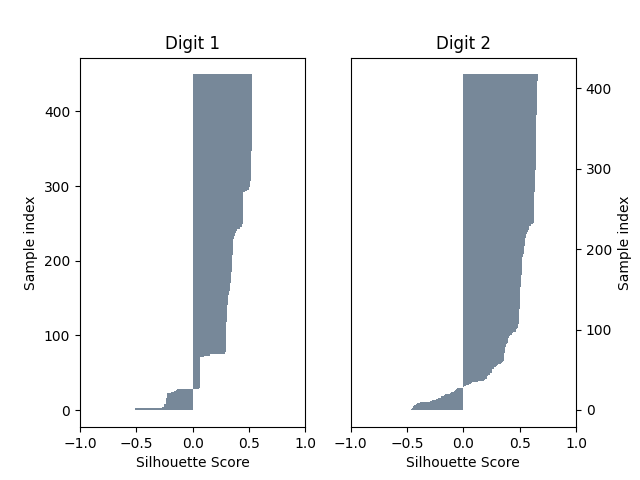
\includegraphics[width=.7\linewidth]{Denoising/s_score1-2_denoising5.png}
	}}\\
	\subfloat[][Train B: $s_\textup{avg} = 0.44\qquad\textup{Loss}_\textup{val} = 0.034$ \label{fig:trainB_s}
	]{
	\resizebox{\linewidth}{!}{
  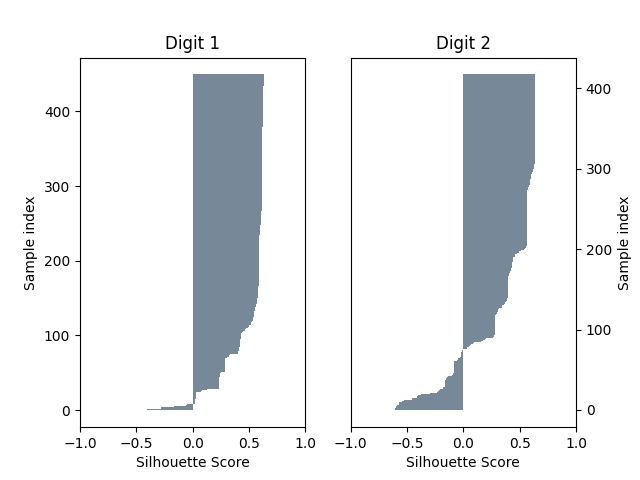
\includegraphics[width=.7\linewidth]{Denoising/s_score1-2_denoising7.png}
	}}
  \caption{Silhouette plots for two different trainings of the denoising autoencoder}
  \label{fig:s_score}
\end{figure}


\begin{figure}
  \subfloat[][Train A: $s_\textup{avg} = 0.41\qquad\textup{Loss}_\textup{val} = 0.034$ \label{fig:trainA_scatter}
	]{
	\resizebox{\linewidth}{!}{
  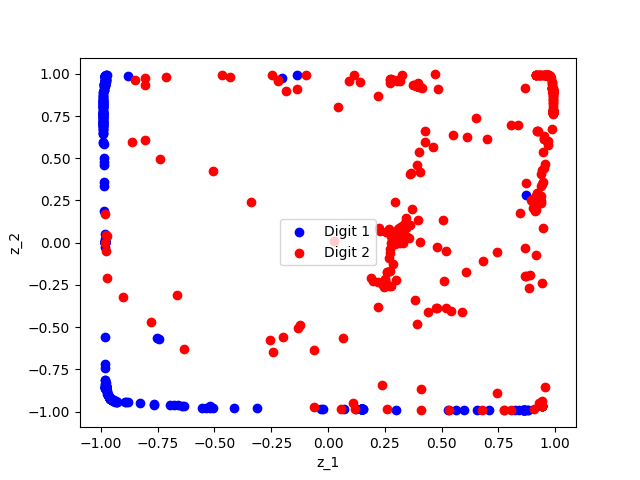
\includegraphics[width=.7\linewidth]{Denoising/scatter1-2_denoising5.png}
  }}\\[-2ex]
	\subfloat[][Train B: $s_\textup{avg} = 0.44\qquad\textup{Loss}_\textup{val} = 0.034$ \label{fig:trainB_scatter}
	]{
	\resizebox{\linewidth}{!}{
  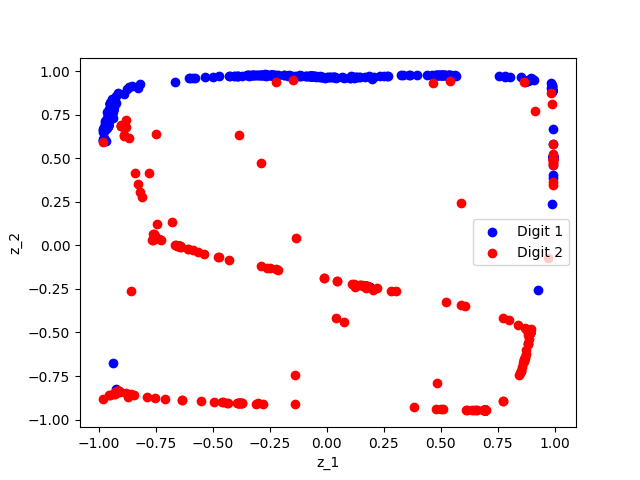
\includegraphics[width=.7\linewidth]{Denoising/scatter1-2_denoising7.png}
	}}
  \caption{Validation data distribution in the latent space with coordinates $(z_1, z_2)$ for two different trainings of the denoising autoencoder (these trainings are the same of fig.~\ref{fig:s_score})}
  \label{fig:scatter}
\end{figure}

PCA produces a latent space where the clustering scores $s_\textup{avg} = 0.47$, a value within the variability observed in the autoencoders.

This section uses only the validation data in order to avoid the pitfall of making assertions on the model using the same data it was trained with. The analysis presented here uses digits 1 and 2. For different couples of digits the results are analogous, a part from those hard to distiguish such as 4 and 9 or 1 and 7, where the denoising autoencoder fails to reconstruct the digits. In the cases were both the normal and denoising autoencoder manage to reconstruct the image there is no difference in the clustering that manifests over the variability to initial conditions.

\section{Conclusions}
The latent space representation shows some structure, but the variability observed with respect to initial conditions suggests that it is merely the autoencoder trying to find an efficient representation, there is no evidence of any sort of convergence to some preferred representation, even on the same model trained with the same hyperparameters. Therefore, the suggestion is that the encoding procedure tends to provide the latent space with a structure that has little to do with the expected data manifold. On the other hand we get the insight that there are many different representations, that there is no reason to believe equivalent. 

In build an efficient representation the activation function can be relevant, hard cut offs such as the one in ReLU can hinder the ability of the net in providing the latent space of this cluster structure. 

As far as this analysis goes there is no manifest advantage in choosing a normal autoencoder or the denoising version. Surprisingly, their performance in the explored task brings no significant advantage from the linear encoding provided by PCA. Even if PCA's ability to reconstruct the correct image is significantly inferior to theirs. However, this is believed to be an accident of the particular setup choosen.

The last result is that the score $s_\textup{avg}$ doesn't seem to vary as strongly as the latent representation with respect to the initial conditions of the training.

\section{Future developments}
There question posed cannot possibly be reduced to the study conducted here which is inherently flawed in many aspects. One such limitation regards the metrics used to choose the model for the analysis. The loss on the validation set does not take into account the cases were the reconstructed image is more similar to the other class than the original label. This criterion is arguably more relevant than the validation loss itself, since the whole analysis revolves around the latent space organization of the data and a wrong \emph{recostruction of the label} (this is the metric proposed) is expected to imply a mispositioning in the latent representation.

Another critical aspect of the problem is the dimensionality of the latent space. The choice of taking it 2-dimensional is due to the argument that each figure has to live at least in a 2-dimensional space, since it has to take into account for rotations and stretches of the image. This is of course an approximation, since for a single label there is a higher variability that cannot be reduced to the aformentioned transformations. Therefore, a proper study across different latent space dimensions is certainly encouraged since one might expect the data manifold to be more approximated better in a higher dimensional latent space.

One further interesting discussion would relate the machine learning methods explored here with more controlled algorithms of manifold identification. There exist many different non linear methods of manifold approximation that rely on geometrical arguments. An interesting one is named \emph{Manifold Sculpting} \cite{Gashler2007}, whose objective is to transform the data while trying to preserve local relations such as distances and angles between neighbor points. This has been part of the original explorative analysis in this work of the different representations of the latent space, in the repository \url{https://github.com/jlancione/DeepLearningProject}
there is a single core implementation\footnote{Pseudocode in the paper \cite{Gashler2007} and reference implementation in the repository \url{https://github.com/Gabriele-Codega/Manifold_Sculpting}.
} in PyTorch of such algorithm but its computational complexity made it unfeasible to conduct a proper analysis with the available resources. 



%\bibliographystyle{plain}  
%\bibliography{Zotero} % Nn trova qlo di Gashler (ha 1 icona diversa...)

\begin{thebibliography}{99}
  \bibitem{Kingma2022}
  Kingma, D. P. \& Welling, M. Auto-Encoding Variational Bayes. Preprint at https://doi.org/10.48550/arXiv.1312.6114 (2022).

  \bibitem{Gashler2007}
  Gashler, M., Ventura, D. \& Martinez, T. Iterative Non-linear Dimensionality Reduction with Manifold Sculpting. in Advances in Neural Information Processing Systems vol. 20 (Curran Associates, Inc., 2007).

  \bibitem{Plaut2018}
  Plaut, E. From Principal Subspaces to Principal Components with Linear Autoencoders. Preprint at https://doi.org/10.48550/arXiv.1804.10253 (2018).

  \bibitem{Rousseeuw1987}
  Rousseeuw, P. J. Silhouettes: A graphical aid to the interpretation and validation of cluster analysis. Journal of Computational and Applied Mathematics 20, 53–65 (1987).
\end{thebibliography}











\end{document}
